\chapter{Vorbereitende Datenbearbeitung}

\section{Prüfen der Datenqualität}
Vor einer Analyse der Messreihen muss immer eine kritische Bewertung der Datenqualität erfolgen. Wenn nötig, müssen Korrekturen vorgenommen werden oder Messdaten aufgrund mangelnder Qualität verworfen werden. Die Bewertung der Datenqualität erfolgt meist visuell. Eine automatische Kontrolle ist jedoch wünschenswert. Die Kriterien für die Überprüfung der Datenqualität sind sehr stark von dem Untersuchungsziel abhängig. Es muss z.B. gefragt werden:
\begin{itemize}
\item
Ist die Abtastung adäquat? Die Abtastrate darf nicht zu gering und sollte nicht zu hoch sein. Eine äquidistante Abtastung ist generell zu bevorzugen. Liegt sie nicht vor, kann sie z.B. durch Interpolation hergestellt werden.
\item
Ändert sich die Qualität der Messreihe? Mitunter müssen fehlerhafte Segmente identifiziert und beseitigt werden. Es kann z.B. vorkommen, dass für ein bestimmtes Messintervall fehlerhafte Messwerte oder konstante Messwerte oder Datenlücken vorliegen. Oft sind auch nur einzelne Werte fehlerhaft (Ausreißer). Sie müssen identifiziert und beseitigt werden.
\item
Wesentlich ist, das SNR zu prüfen. Ist das Signal überhaupt zu erkennen? Lohnt sich eine Bearbeitung der Daten?
\item
Oft gibt es spezielle Fragestellungen. Z.B.: ist die Polarität korrekt? Ist die Orientierung der Komponenten korrekt? Sind die Amplituden korrekt? Gibt es Zeitfehler? Zeitfehler sind oft schwer zu erkennen, können aber z.B. durch die Drift der internen Uhr (Beispiel Ozeanbodenseismometer) auftreten. Mitunter hilft ein Vergleich von markanten Signalen, die an der zu untersuchenden und einer Referenzstation registriert worden sind, um Zeitfehler zu erkennen. Auch die mittels ambient noise berechnete Greensfunktion kann für das Erkennen der Zeitdrift verwendet werden. Relative Laufzeiten sind unabhängig von der Fehlern in der absoluten Zeit und können verwendet werden, falls eine zuverlässige Korrektur des Zeitfehlers nicht möglich ist.    
\end{itemize}
Eine Verbesserung der Datenqualität kann mitunter durch einfaches Entfernen fehlerhafter Daten erfolgen, mitunter muss ein anspruchsvolle und optimierte Signalverarbeitung erfolgen. 

\section{Einfache Transformationen}

\section{Trendbestimmung und -korrektur}
Einer der ersten Schritte der Signalverarbeitung ist die Bestimmung des Trends. Der Trend kann sowohl Nutz- wie Störsignal sein. Um ihn bestimmen zu können, wird ein Modell angenommen:
\[
x_i=m_i + y_i, i=1,\dots, N
\]
 dabei ist $x_i$ die betrachtete Wertereihe, die sich aus dem Trend $m_i$ und einem überlagerten Signal $y_i$ zusammensetzt. Im Fall der Seismik oder Seismologie ist ${y_i}$ das Nutzsignal und der Trend soll bestimmt und beseitig (korrigiert) werden. Für die Entwickung der Bevölkerungszahl oder für Börsenkurse ist ${m_i}$ das interessierende Phänomen und ${y_i}$ würde als Rauschen bezeichnet werden können.\\\\
Eine Möglichkeit den Trend zu bestimmen ist, ein Modell für den Trend anzunehmen und dessen Parameter zu schätzen. Oft wird für den Trend das Modell eines Polynoms gewählt:
\[
m_i(a_j)=a_0+ a_1t_i+a_2t_i^2+\dots = \sum\limits_{j=0}^{q} a_j t_i^j
\]
Dbei sind ${a_j}$ die Koeffizienten des Polynoms, welche nach der Methode der kleinsten Quadrate bestimmt werden können. Dabei wird die Fehlerquadratsumme $E$ minimiert:
\[
E=\sum\limits_{i=0}^N (x_i -m_i)^2 \rightarrow \mbox{Min.}
\]
D.h. für die Koeffizienten soll gelten:
\[
\frac{\partial E}{\partial a_k}\stackrel{!}{=}0
\]
Diese Bedingung liefert für ein lineares Modell ein lineares Gleichungssystem zur Bestimmung der Parameter. Die Lösung des Gleichungssystems liefert dann die Schätzungen $\hat{a_k}$, mit denen der Trend des Signals gesschätzen werden kann: $m_i(\hat a_k)$. Die trendkorrigierte Wertereihe ist dann:
\[
\hat{y_i}=x_i-m_i(\hat a_k)
\]
Zu beachten ist, dass das Zeitfenster und die Ordnung $q$ geeignet gewählt werden müssen. Die Ordung $q$ sollte möglichst klein (z.B. 1.-Ordnung für einen linearen Trend) gewählt und wenn nötig schrittweise erhöht werden. Die Ordnung muss so klein sein, dass das $m(\hat a_k)$ nicht Anteile von ${y_i}$ enthält. Das Zeitfenster sollte eher lang als zu kurz gewählt werden. Möglicherweise kann der Trend auch in einem Zeitfenster vor dem Einsetzen eines Signals bestimmt werden.\\\\

\subsection{Moving Average}
Der Trend kann auch mittels Filterung oder eines \textsl{Moving Average} (gleitendes Mittel, MA) bestimmt werden.\\\\
Ein \textit{akausales}, zweiseitiges hat eine Länge von $2q + 1$. Dabei wird auch auf zukünftige Werte zugegriffen, die Bearbeitung kann also nur \textbf{offline} erfolgen.
\begin{equation}
\hat{m_i}=(2q+1)^{-1}\sum\limits_{j=-q}^q x_{i-j}
\end{equation}
Für ein \textit{kausales}, einseitiges gleitendes Fenster wird nur auf aktuelle und vergangene Werte zugegriffen. Diese Variante ist geeignet für die Bestimmung des Trends in Echtzeit (\textbf{online}). Allerdings fürht dies zu einer Phasenverschiebung der Signale.
\begin{equation}
\hat{m_i}=(q+1)^{-1}\sum\limits_{j=0}^q x_{i-j}
\end{equation}

Das gleitende Mittel kann auch rekursiv bestimmt werden
\begin{equation}
\hat m_i=(q+1)^{-1} x_i +  \hat m_{i-1}-(q+1)^{-1} x_{i-1-q}
\end{equation}
Dabei ist $x_i$ der aktuelle Wert in der Signalreihe. Setzt man $x_{i-1-q}\stackrel{!}{=}\hat m_{i-1}$ werden nur $\hat m_{i-1}$ und $x_i$ benötigt
\begin{equation}
\hat{m_i}= \alpha x_i + (1-\alpha) \hat m_{i-1}
\end{equation}
{\small mit $\alpha = (q+1)^{-1}$}\\
Diese Näherung ist sehr einfach zu berechnen. Sie ist nicht exakt, aber oft ausreichend.\\\\
In einem gleitenden Fenster können statt dem Mittelwert auch Quantile geschätzt werden. Quantile $Q_p$ ist der Wert $s$, für den die Verteilungsfunktion $\underline P(s)=p$ ist. $Q_{0.5}$ ist der Median, $Q_{0.25},Q_{0.5},Q_{0.75}$ sind Quartile der Verteilung.

\section{Saisonale Komponenten}
Interessant ist auch der Fall, in dem eine periodischer Anteil (saisonale Komponente) bestimmt werden und möglicherweise beseitigt werden sollen.
\[
x_i=s_i + y_i
\]
{\small Dabei ist $x_i$: Wertereihe, $s_i$: saisonale Komponente (z.B. Jahres-, Tagesgang, 60 Hz Stromnetz oder Milankovic-Zyklen) und $y_i$: Signalreihe.}\\\\
Mögliche Methoden um die Saisonale Komponente Im Signal zu erfassen:

\begin{enumerate}
\item Kann man die Signalreiehe Differenzieren oder Filtern? Hilft es das Spektrum berechnen, um Frequenzen der saisonalen Komponente zu erkennen.

\item Moving Avarage $d$, die Periode von $s_i$ ist bekannt. Ein $q$ wählen, so dass $d=2q+1$\\
{\color{red}????? was ist hiermit gemeint}

\item Ein Modell für saisonale Komponenten annehmen, Parameter bestimmen, $\hat s_i$ schätzen und von $x_i$ abziehen.

\paragraph{Beispiel} Externe Messung einer Störgröße $p_i$. Als Modell kann im einfachsten Fall $s_i=f(p_i) = ap_i$ angenommen und $a$ nach der Methode der kleinsten Quadrate bestimmen bestimmt werden kann. Hier kann $x_i$ z.B. eine kontinuierliche Schweremessung und $p_i$ eine Messung des Luftdrucks sein. 

\paragraph{Beispiel} Ein etwas komplizierteres Modell ist die Überlagerung von Cosinus-Funktionen verschiedener Frequenz.
\[
s_i=\sum\limits_{j=0}^N a_j \cos(w_jt_i+\varphi_j)
\]
{\small Wobei $a_j$,$\varphi_j$: unbekannt; $\omega_j$: bekannt}\\
Mithilfe des Additionstheorems und lösung dessen können die unbekannten Schwingungen identifiziert werden.
\[
s_i=\sum\limits_{j=0}^N a_j (\cos(w_jt_i)\cos(\varphi_j) - \sin(w_jt_i) \sin(\varphi_j))
\]
{\small Wobei die Phase der Signale $\phi$ unbekannt ist}\\
Die Gleichung kann umformuliert werden zu:
\[
s_i=\sum\limits_k c_k b_{ki}
\]
Dabei ist
\[
b_{ki}=
\begin{pmatrix}
\cos(\omega_1t_i)\\
\vdots \\
\cos(\omega_qt_i \\
-\sin(\omega_1t_i)\\
\vdots \\
-\sin(\omega_qt_i
\end{pmatrix}
; c_k=
\begin{pmatrix} 
a_1 \cos(\varphi_1)\\
a_2 \cos(\varphi_2)\\
\vdots\\
a_1 \sin(\varphi_1) \\
a_2 \sin(\varphi_2)
\end{pmatrix}
\]
Mithilfer der Methode der Kleinsten Quadrate Lösen wir:
\[
E = \sum\limits_i (x_i- \sum\limits_j c_j b_{ji})^2
\]
zu
\[
\sum\limits_i x_i b_{ki} = \sum\limits_j c_j\sum\limits_i b_{ji}b_{ki}
\]
Rechte Seite einer Bestimmungsgleichung ist die Projektion der Messwerte auf Basisfunktionen
Weiter gilt:
\[
a_j=(c_j^2+c_{j+a}^2)^{0.5}, \varphi_j=\arctan(\frac{c_{j+a}}{c_j})
\]

\paragraph{Beispiel} $s_i=a \cos(\omega t + \varphi)$; wobei zusätzlich zu $a$ und $\varphi$ auch die Frequenz $\omega$ unbekannt ist. Durch die unbekannte Frequenz wird das Problem nicht-linear. Es müssen Methoden der nicht-lineare Optimierung genutzt werden, um die Parameter $\omega, a$ und $\varphi$ zu bestimmen.
\end{enumerate}

\section{Resampling einer Signalreihe}
Will man den Abtastschritt (\textsl{Samplingrate}) einer schon aufgezeichneten Zeitereihe ändern kann die Interpolation des Signals im Frequenz oder Zeitbereich durchgeführt werden.

\subsection{Interpolation im Zeitbereich}
Im Zeitbereich kann der Abtastschritt einer diskreten Signalreihe durch harmonisch überlagernde $Sinc$ Funktionen erhöht werden.
\begin{equation}
x(t) = \sum_{j=0}^{N-1} x(j \Delta t) \, \mbox{sinc} \left(\omega_{Ny}(t-{t_j}\right)
\end{equation}
Die Superposition der Sinc Funktionen ist jeweils um $t_j$ verschoben und je mit der gemessenen Amplitude $x(j\Delta t)$ gewichtet.

\begin{figure}[h!]
\centering
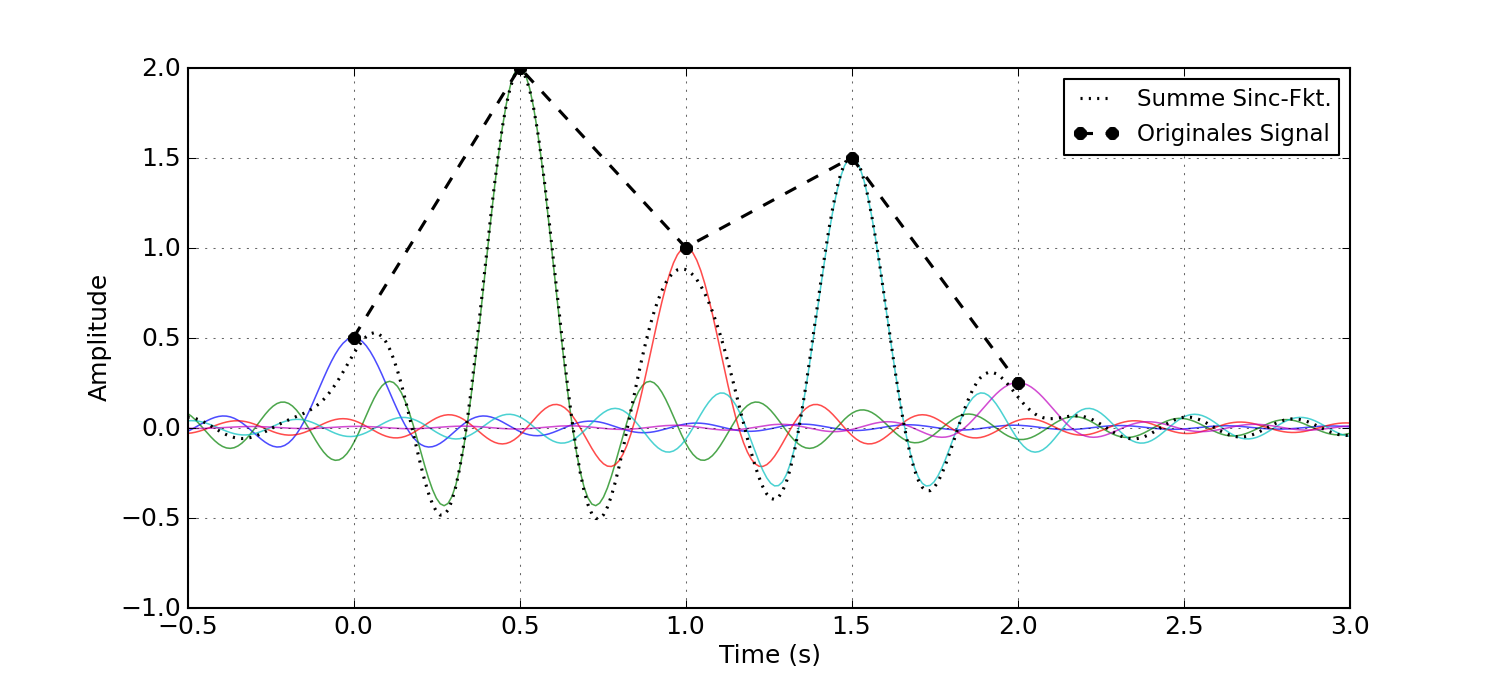
\includegraphics[width=.9\tw]{fig/04-Daten/interpolation_sinc.png}
\caption{Interpolation im Zeitbereich durch gewichtete und überlagernde Sinc Funktionen.}
\end{figure}
